\chapter{Sistema di testing}

\section{Sistema di testing}
\paragraph{Traccia}
Progettare, implementare in VHDL e verificare mediante simulazione un sistema in grado di testare in maniera automatica una macchina combinatoria M avente 4 ingressi e 3 uscite binarie sottoponendole N ingressi diversi (si considerino una macchina M e un numero di input N a scelta dello studente). 
Gli N valori di input per il test devono essere letti da una ROM, in cui essi sono precaricati, in corrispondenza di un segnale read. Le N uscite fornite della macchina in corrispondenza di ciascuno degli input devono essere memorizzate in una memoria interna, che deve poter essere svuotata in qualsiasi momento in presenza di un segnale di reset.


\subsection{Architettura}
L'architettura della soluzione è illustrata in Figura \ref{fig:Architettura sistema di testing} ed è composta dai seguenti componenti:
\begin{itemize}
    \item \textit{ROM}: memoria di sola lettura che contiene gli ingressi da inviare alla macchina combinatoria;
    \item \textit{Macchina combinatoria}: macchina che riceve un ingresso a 4 bit e offre un uscita a 3 bit;
    \item \textit{Memoria}: si occupa di memorizzare il risultato delle operazioni in uscita dalla macchina combinatoria;
    \item \textit{Rete di controllo}: si occupa di gestire la tempificazione della macchina fornendo i segnali di scrittura e indirizzo alle memorie;
\end{itemize}

\begin{figure}[H]
    \centering
    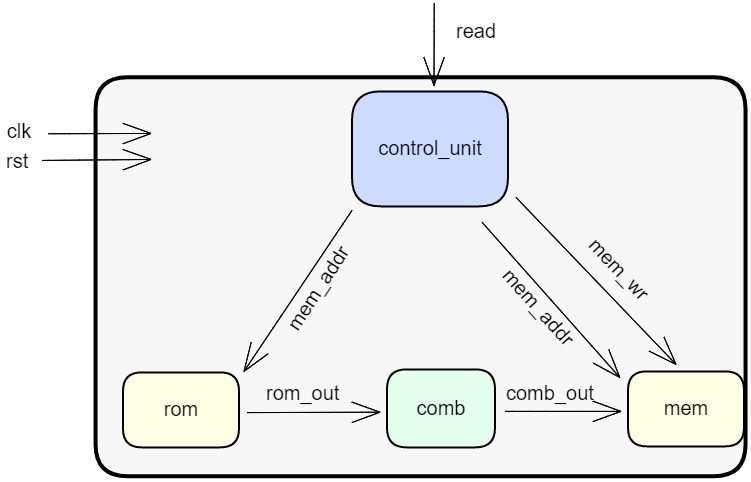
\includegraphics[width=15cm]{immagini/esercizio6/schema_6.1.png}
    \caption{Architettura sistema di testing}
    \label{fig:Architettura sistema di testing}
\end{figure}

\paragraph{Rete di controllo}
La rete di controllo è stata implementata attraverso l'automa a stati finiti illustrato in Figura \ref{fig:fsm_6}. Il sistema si predispone alla memorizzazione del risultato della macchina combinatoria ponendo \textit{mem\_wr=1} nello stato \textit{load} e poi si blocca in attesa del segnale di \textit{read} nello stato \textit{wait\_read}. Infine, lo stato \textit{ctrl} serve a rendere consistente l'incremento del segnale di indirizzo \textit{mem\_addr}.

\begin{figure}[H]
    \centering
    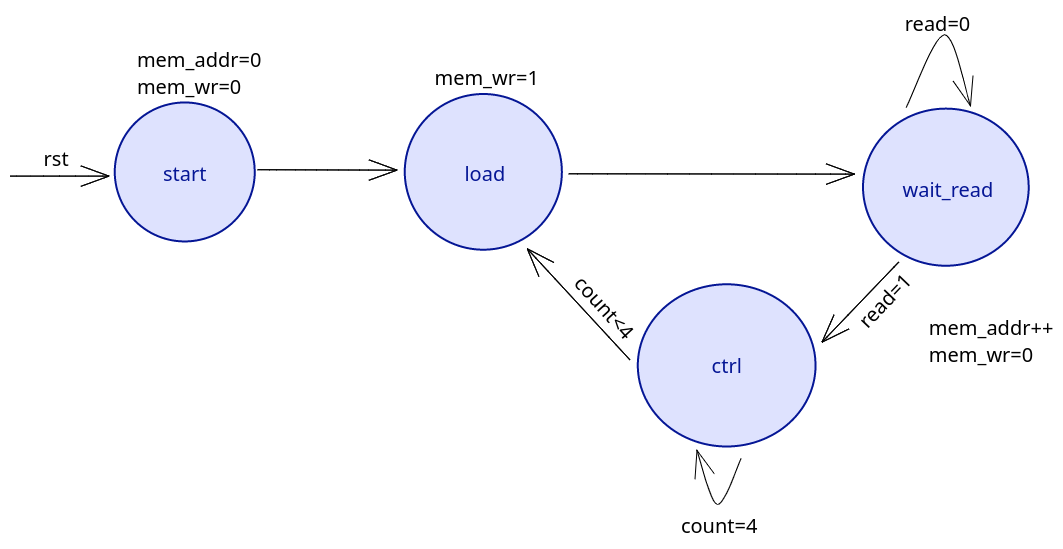
\includegraphics[width=16cm]{immagini/esercizio6/automa_6.1.png}
    \caption{Automa a stati finiti}
    \label{fig:fsm_6}
\end{figure}

Nel listato \ref{fsm_6} è mostrata l'implementazione dell'automa in Figura \ref{fig:fsm_6}.

\begin{lstlisting} [language=VHDL,label=fsm_6, caption=Implelemtazione automa a stati finiti] 
library IEEE;
use IEEE.STD_LOGIC_1164.ALL;
use ieee.numeric_std.all ;

entity rete_di_controllo is
    Port (
        clk,reset,read: in std_logic ;
        addr: out std_logic_vector (1 downto 0);
        write: out std_logic

    );
end rete_di_controllo;

architecture Behavioral of rete_di_controllo is

    type state is (
        START,
        LOAD,
        WAIT_READ,
        CTRL
    );
    signal current_state : state:= START;
    signal next_state : state;
    signal s_addr: std_logic_vector (1 downto 0);
begin
    comb: process(current_state,read)
    variable count: integer:=0;

    begin
        case current_state is
        
            when START =>
                s_addr<="00";
                write<='0';
                count:=0;
                next_state<= LOAD ;
                
            when LOAD  =>
                next_state<= WAIT_READ ;
                write<='1';
 
            when WAIT_READ  =>
                if (read='1') then
                    next_state<= CTRL  ;
                    write<='0';
                    s_addr <= std_logic_vector((unsigned(s_addr) + 1));
                    count:=count+1;
                else
                    next_state<= WAIT_READ ;
                end if;

            when CTRL =>
                if (count=4)then
                   next_state<= CTRL ;
                else 
                   next_state<= LOAD;
                end if;

            when others =>
                next_state<= START;
        end case;
    end process;
    
addr<=s_addr ;

    seq: process(clk)
    begin
        if rising_edge(clk) then
            if reset='1' then
                current_state<=START;
            else
                current_state<=next_state;
            end if;
        end if;
    end process seq;

end Behavioral;

\end{lstlisting}


\paragraph{Rom}
La rom è stata implementata con un processo ed è rappresentata da un \textit{array} di vettori da $3$ bit. In particolare, è stata scelta un'implementazione \textit{single port} con lettura asincrona. Nel listato \ref{rom_6} è mostrata l'implementazione della rom.

\begin{lstlisting}[language=VHDL,label=rom_6, caption=Implelemtazione automa a stati finiti]
library ieee;
use ieee.std_logic_1164.all;
use ieee.numeric_std.all;

entity rom is
port(
    clk, read : in std_logic; 
    addr : in std_logic_vector(1 downto 0);
    data : out std_logic_vector(3 downto 0)
    );
end rom;

architecture behavioral of rom is 
type rom_type is array (0 to 3) of std_logic_vector(3 downto 0);
signal ROM : rom_type := (
    "0001", 
    "0110", 
    "1011", 
    "1111"
);

begin

process(clk)
  begin
    if rising_edge(clk) then
          data <= rom(to_integer(unsigned(addr)));
    end if;
end process;
end behavioral;
\end{lstlisting}

\paragraph{Macchina combinatoria}
La macchina combinatoria scelta effettua un'operazione molto semplice che trasforma un ingresso a $4$ bit in uscita a $3$ bit. In particolare, dato un ingresso $X=X_3X_2X_1X_0$, l'uscita $Y$ si ottiene nel seguente modo:
\begin{equation*}
    Y = (X_3\;AND\;X_2)\;\&X_1\;\&\;X_0
\end{equation*}
dove con il simbolo $\&$ si indica l'operazione di concatenamento.
 
\begin{lstlisting} [language=VHDL, caption=Macchina combinatoria]
library IEEE;
use IEEE.STD_LOGIC_1164.ALL;

entity macchina_combinatoria is
    port(
        input: in std_logic_vector(3 downto 0);
        output: out std_logic_vector( 2 downto 0)
    );
end macchina_combinatoria;

architecture behavioral of macchina_combinatoria is

begin
    output <= (input(3)and input(2)) & input(1) & input(0);
end behavioral;

\end{lstlisting}

\paragraph{Memoria}
In maniera simile alla ROM, la memoria è implementata con un approccio comportamentale. In particolare, è stata scelta una memoria \textit{single-port} con lettura asincrona effettua la scrittura in corrispondenza del segnale di ingresso \textit{write}. Nel listato \ref{memoria}, è riportata l'implementazione della memoria.
\begin{lstlisting} [language=VHDL, label=memoria, caption=Implementazione memoria]
library ieee;
use ieee.std_logic_1164.all;
use ieee.std_logic_unsigned.all;

entity memoria is
port(
    clk, read, write, reset : in std_logic; 
    addr : in std_logic_vector(1 downto 0);
    input : in std_logic_vector(2 downto 0);
    output : out std_logic_vector(2 downto 0)
    );
end memoria;

architecture behavioral of memoria is 
type memoria_type is array (0 to 3) of std_logic_vector(2 downto 0);
signal MEM : memoria_type := (
    "000", 
    "000", 
    "000", 
    "000"
);

begin
    process(clk)
      begin
        if rising_edge(clk) then
            if reset = '1' then
                 for i in 0 to 3 loop 
                     MEM(i) <= "000";
                 end loop;
            elsif write = '1' then
                MEM(conv_integer(addr)) <= input;        
            end if;
        end if;
        output<=MEM(conv_integer(addr));   
    end process;
end behavioral;
\end{lstlisting}

\paragraph{Sistema complessivo} Il sistema complessivo è stato assemblato a partire dai componenti descritti in precedenza e collegati in maniera opportuna. In particolare, attraverso il segnale \textit{mem\_addr} la rete di controllo si interfaccia con la ROM e la memoria. Quest'ultima riceve anche il segnale di \textit{write} per la scrittura. Inoltre, attraverso il segnale \textit{s\_data}, l'uscita della ROM è collegata in ingresso alla macchina combinatoria; mentre la sua uscita è collegata in ingresso alla memoria mediante il segnale \textit{s\_output}. Nel listato \ref{sis_6_1}, è mostrato il sistema complessivo.

\begin{lstlisting} [language=VHDL, label=sis_6_1, caption=Sistema complessivo]
library IEEE;
use IEEE.STD_LOGIC_1164.ALL;

entity test_automatico is
  Port ( 
    clk, reset, read: in std_logic;
    out_123: out std_logic_vector(2 downto 0)
  );
end test_automatico;

architecture structural of test_automatico is

component macchina_combinatoria is
    port(
        input: in std_logic_vector(3 downto 0);
        output: out std_logic_vector( 2 downto 0)
    );
end component macchina_combinatoria;

component memoria is
port(
    clk, read, write, reset : in std_logic; 
    addr : in std_logic_vector(1 downto 0);
    input : in std_logic_vector(2 downto 0);
    output : out std_logic_vector(2 downto 0)
    );
end component memoria;

component rom is
port(
    clk, read : in std_logic; 
    addr : in std_logic_vector(1 downto 0);
    data : out std_logic_vector(3 downto 0)
    );
end component rom;

component rete_di_controllo is
    port(
    clk,reset,read: in std_logic;
    write: out std_logic;
    addr: out std_logic_vector(1 downto 0) 
);
end component rete_di_controllo;

signal s_write : std_logic := '0';
signal s_addr : std_logic_vector(1 downto 0) := "00";
signal s_data: std_logic_vector(3 downto 0) := "0000";
signal s_output: std_logic_vector(2 downto 0) := "000";
begin

MC: macchina_combinatoria port map(
      input=>s_data,
      output=>s_output
);

M: memoria port map (
    clk=>clk,
    read=>read,
    write=>s_write,
    addr=>s_addr,
    reset=>reset,
    input=>s_output,
    output=>out_123
);

R: rom port map (
 clk=>clk,
 read=>read,
 addr=>s_addr,
 data=>s_data
);

RC: rete_di_controllo port map(
    clk=>clk,
    read=>read,
    write=>s_write,
    reset=>reset,
    addr=>s_addr
);

end structural;
\end{lstlisting}

\subsection{Testing}
Il sistema è stato testato fornendo in ingresso 4 segnali di \textit{read} distinti. In uscita, come mostrato nella simulazione in Figura \ref{fig:sim_6.1}, ad ogni \textit{read}, l'uscita commuta correttamente con il risultato della macchina combinatoria. Il \textit{testbench} è riportato nel listato \ref{tb_sis_6.1}.

\begin{lstlisting} [language= VHDL, label=tb_sis_6.1, caption=Testbench sistema complessivo]
library IEEE;
use IEEE.STD_LOGIC_1164.ALL;

entity test_automatico_tb is
end test_automatico_tb;

architecture Behavioral of test_automatico_tb is

    component test_automatico is
        Port (
            clk, reset, read: in std_logic;
            out_123: out std_logic_vector(2 downto 0)
        );
    end component test_automatico;

    signal s_clk, s_reset, s_read : std_logic := '0';
    signal s_output:  std_logic_vector(2 downto 0):="000";
    constant clk_period: time := 10 ns;
begin

    uut: test_automatico port map(
            clk=>s_clk,
            reset=>s_reset,
            read=>s_read,
            out_123=>s_output
        );

    clock: process
    begin
        s_clk <= not s_clk;
        wait for clk_period/2;
    end process clock;

    sus: process
    begin
        wait for 100ns;
        s_reset <='1';
        wait for clk_period;
        s_reset <='0';
        wait for 5*clk_period;

        s_read <= '1';
        wait for clk_period;
        s_read <= '0';
        wait for 5*clk_period;

        s_read <= '1';
        wait for clk_period;
        s_read <= '0';
        wait for 5*clk_period;

        s_read <= '1';
        wait for clk_period;
        s_read <= '0';
        wait for 5*clk_period;

        s_read <= '1';
        wait for clk_period;
        s_read <= '0';
    wait;
    end process sus;
end Behavioral;


\end{lstlisting} 

\begin{figure}[H]
    \centering
    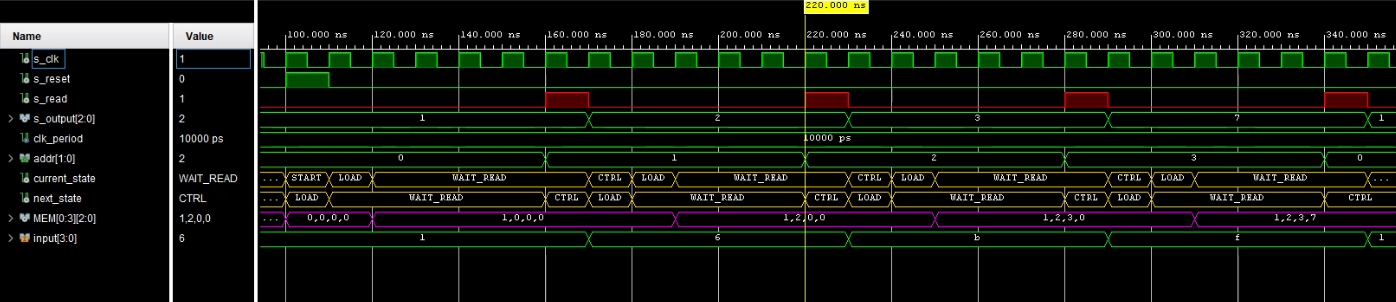
\includegraphics[width=15cm]{immagini/esercizio6/output_simulazione_6.1.png}
    \caption{Simulazione esercizio 6.1}
    \label{fig:sim_6.1}
\end{figure}

\section{Sintesi su scheda}
\paragraph{Traccia} Sintetizzare ed implementare su board il componente sviluppato al punto precedente, utilizzando due bottoni per i segnali di read e reset rispettivamente e i led per la visualizzazione delle uscite della macchina istante per istante.

\subsection{Implementazione}
Per l'implementazione su \textit{board}, il componente descritto nel paragrafo precedente viene utilizzato da una unità \textit{top} (implementata nel listato \ref{top_6.2}). Questa unità gestisce la comunicazione con la scheda fisica instanziando un \textit{debouncer} per il pulsante di \textit{read} ed effettua il collegamento delle uscite sui led. Una dimostrazione visuale del risultato è disponibile nel file \textit{6.2.mkv} del materiale multimediale.

\begin{lstlisting} [language= VHDL, label=top_6.2, caption=Unità TOP]
library IEEE;
use IEEE.STD_LOGIC_1164.ALL;

entity top is
    Port (
        clock,reset,set: in std_logic ;

        output : out std_logic_vector (2 downto 0)
    );
end top;

architecture Structural of top is
    component ButtonDebouncer is
        generic (
            CLK_period: integer := 10;  -- periodo del clock in nanosec
            btn_noise_time: integer := 10000000 --durata dell'oscillazione in nanosec
        );
        Port ( RST : in STD_LOGIC;
             CLK : in STD_LOGIC;
             BTN : in STD_LOGIC;
             CLEARED_BTN : out STD_LOGIC);
    end component ButtonDebouncer;

    component cu is
        Port (
            clock,reset,read: in std_logic ;
            addr: out std_logic_vector (1 downto 0);
            write: out std_logic
        );
    end component cu;

    component memoria is
        port(
            clk, read, write, reset : in std_logic;
            addr : in std_logic_vector(1 downto 0);
            input : in std_logic_vector(2 downto 0);
            output : out std_logic_vector(2 downto 0)
        );
    end component memoria;

    component rom_sp_sr is
        port(
            clk : in std_logic;
            addr : in std_logic_vector(1 downto 0);
            data : out std_logic_vector(3 downto 0)
        );
    end component;

    component combinatorial is
        Port (
            x: in std_logic_vector(3 downto 0);
            y: out std_logic_vector(2 downto 0)
        );
    end component;

    signal s_set,s_write: std_logic ;
    signal s_rom_out: std_logic_vector (3 downto 0);
    signal s_addr: std_logic_vector (1 downto 0);
    signal s_output:std_logic_vector (2 downto 0);
begin
    rc: cu port map(
            clock=> clock,
            reset=> reset,
            read=> s_set,
            addr=> s_addr,
            write=>s_write
        );
    db: ButtonDebouncer port map(
            RST => reset ,
            CLK => clock ,
            BTN => set,
            CLEARED_BTN => s_set
        );
    mc: combinatorial port map(
            x=>s_rom_out,
            y=>s_output
        );
    output<=s_output;
    r: rom_sp_sr port map(
            clk=>clock ,
            addr=>s_addr ,
            data=> s_rom_out
        );
    M: memoria port map (
            clk=>clock,
            read=>'0',
            write=>s_write,
            addr=>s_addr,
            reset=>reset,
            input=>s_output,
            output=>OPEN
        );
end Structural;
\end{lstlisting}